
\documentclass{exam}

\usepackage{graphicx}
\usepackage[fleqn]{amsmath}
\usepackage{unitsdef} 
\usepackage{cancel}
\usepackage{float}
\usepackage{mdwlist}
\usepackage{booktabs}
\usepackage{cancel}
\usepackage{polynom}
\usepackage{caption}
\usepackage{fullpage}
\usepackage{enumerate}

% \newcommand{\degree}{\ensuremath{^\circ}} 
\everymath{\displaystyle}

\newunit{\inch}{in}
\newunit{\foot}{ft}
\newunit{\cemtimeter}{cm}

% \begin{figure}[H]
%   \centering
%   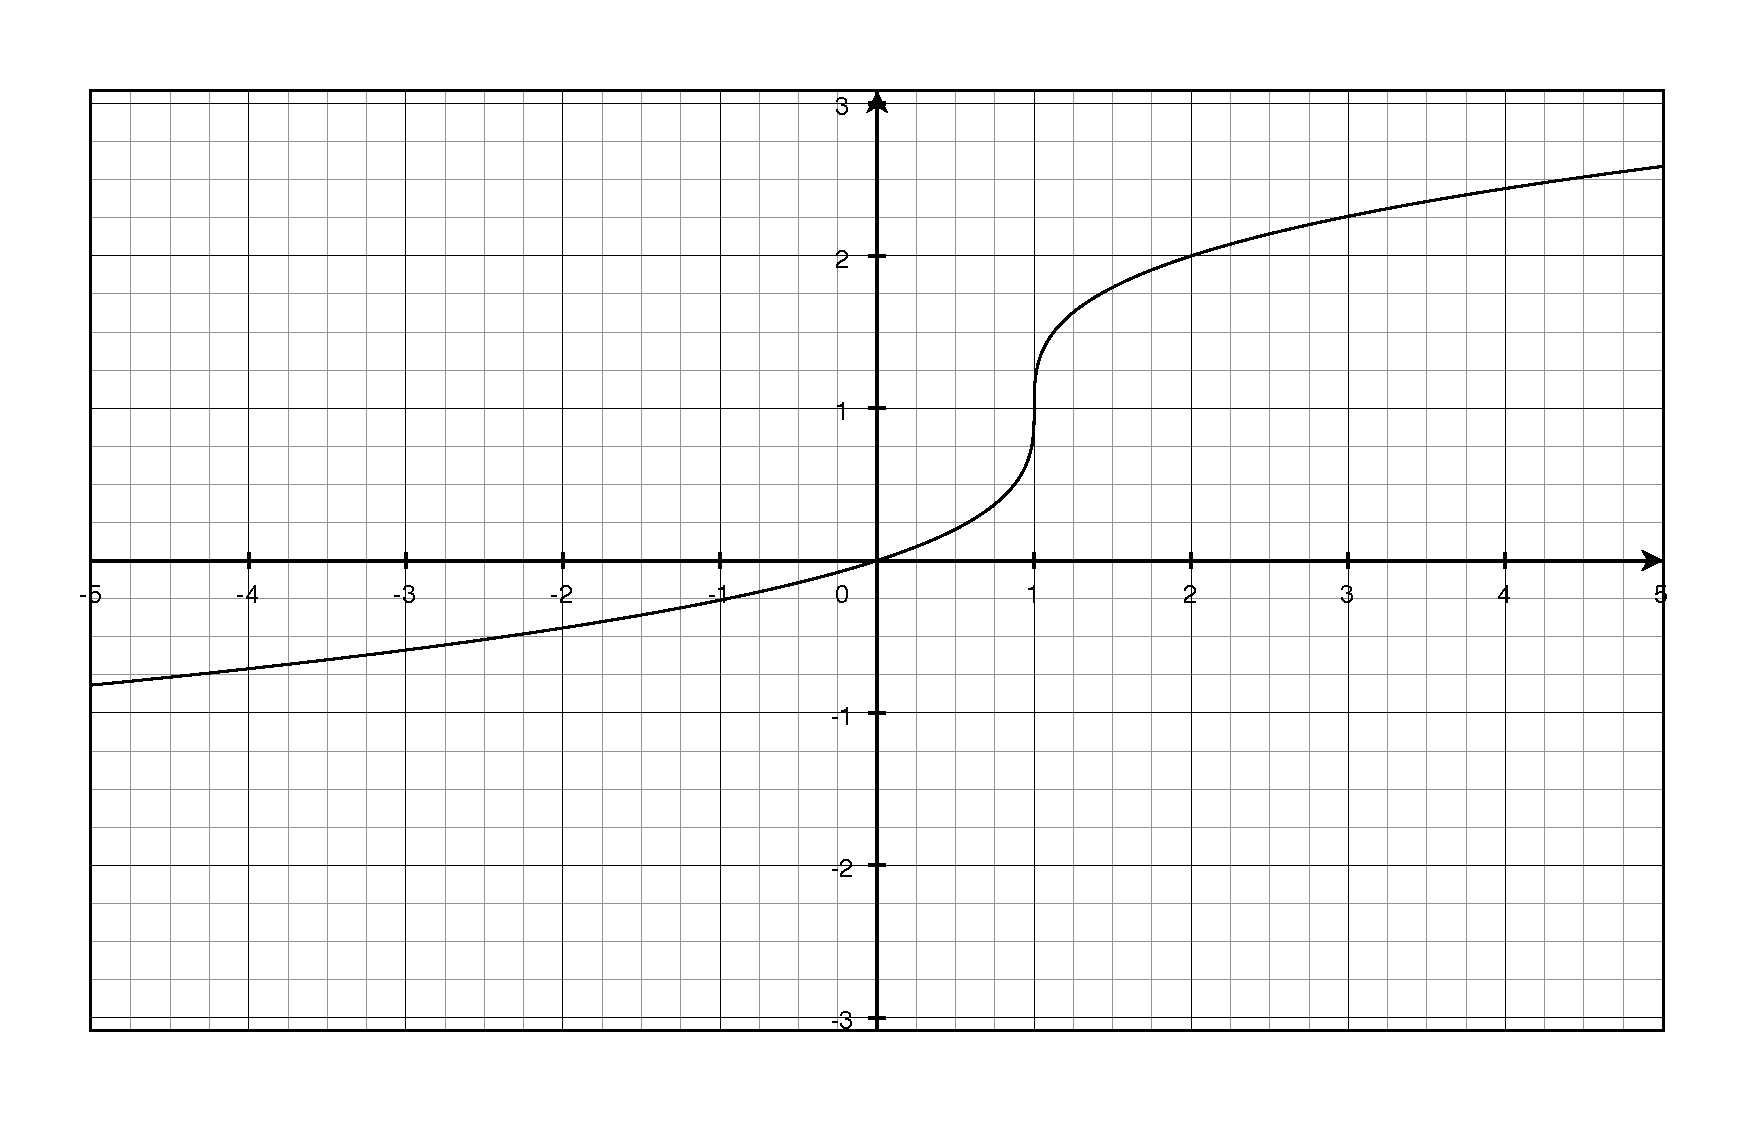
\includegraphics[scale=.3]{question7.eps}
%   \caption*{Question 7}
% \end{figure}

% \begin{tabular}{cc}
% \toprule
% period & amplitude \\
% \midrule
%   $\pi$ & $2$ \\
% \bottomrule
% \end{tabular}

\printanswers

\ifprintanswers 
\usepackage{2in1, lscape} 
\fi

\title{Math 263B \\ Homework Four}
\date{August 2, 2012}

\begin{document}

\maketitle

\ifprintanswers
\else
\section{Notes}

Section 5.5 provides a detailed definition of definite integrals along with a difficult way of calculating them.
Section 5.6 provides a much easier way of doing the calculations.  So I thought we'd not dwell too long on
section 5.5 and focus more on 5.6.  

However, there's quite a bit of material in 5.6, so the plan is:
\begin{itemize*}
  \item this week: 5.5 and first half of 5.6
  \item next week: second half of 5.6 and 5.7
\end{itemize*}
 
\fi

\section{Homework}

\begin{itemize*}
  \item Read Section 5.5 and 5.6
  \item pp 267-269: 7-13, 21
  \item pp 274-275: 1-14, 31-32
\end{itemize*}

\section{Extra Credit}
Find the area between the curves: $y = 5x$, $y = x^2$, $x = 1$, and $x = 4$

\begin{figure}[H]
  \centering
  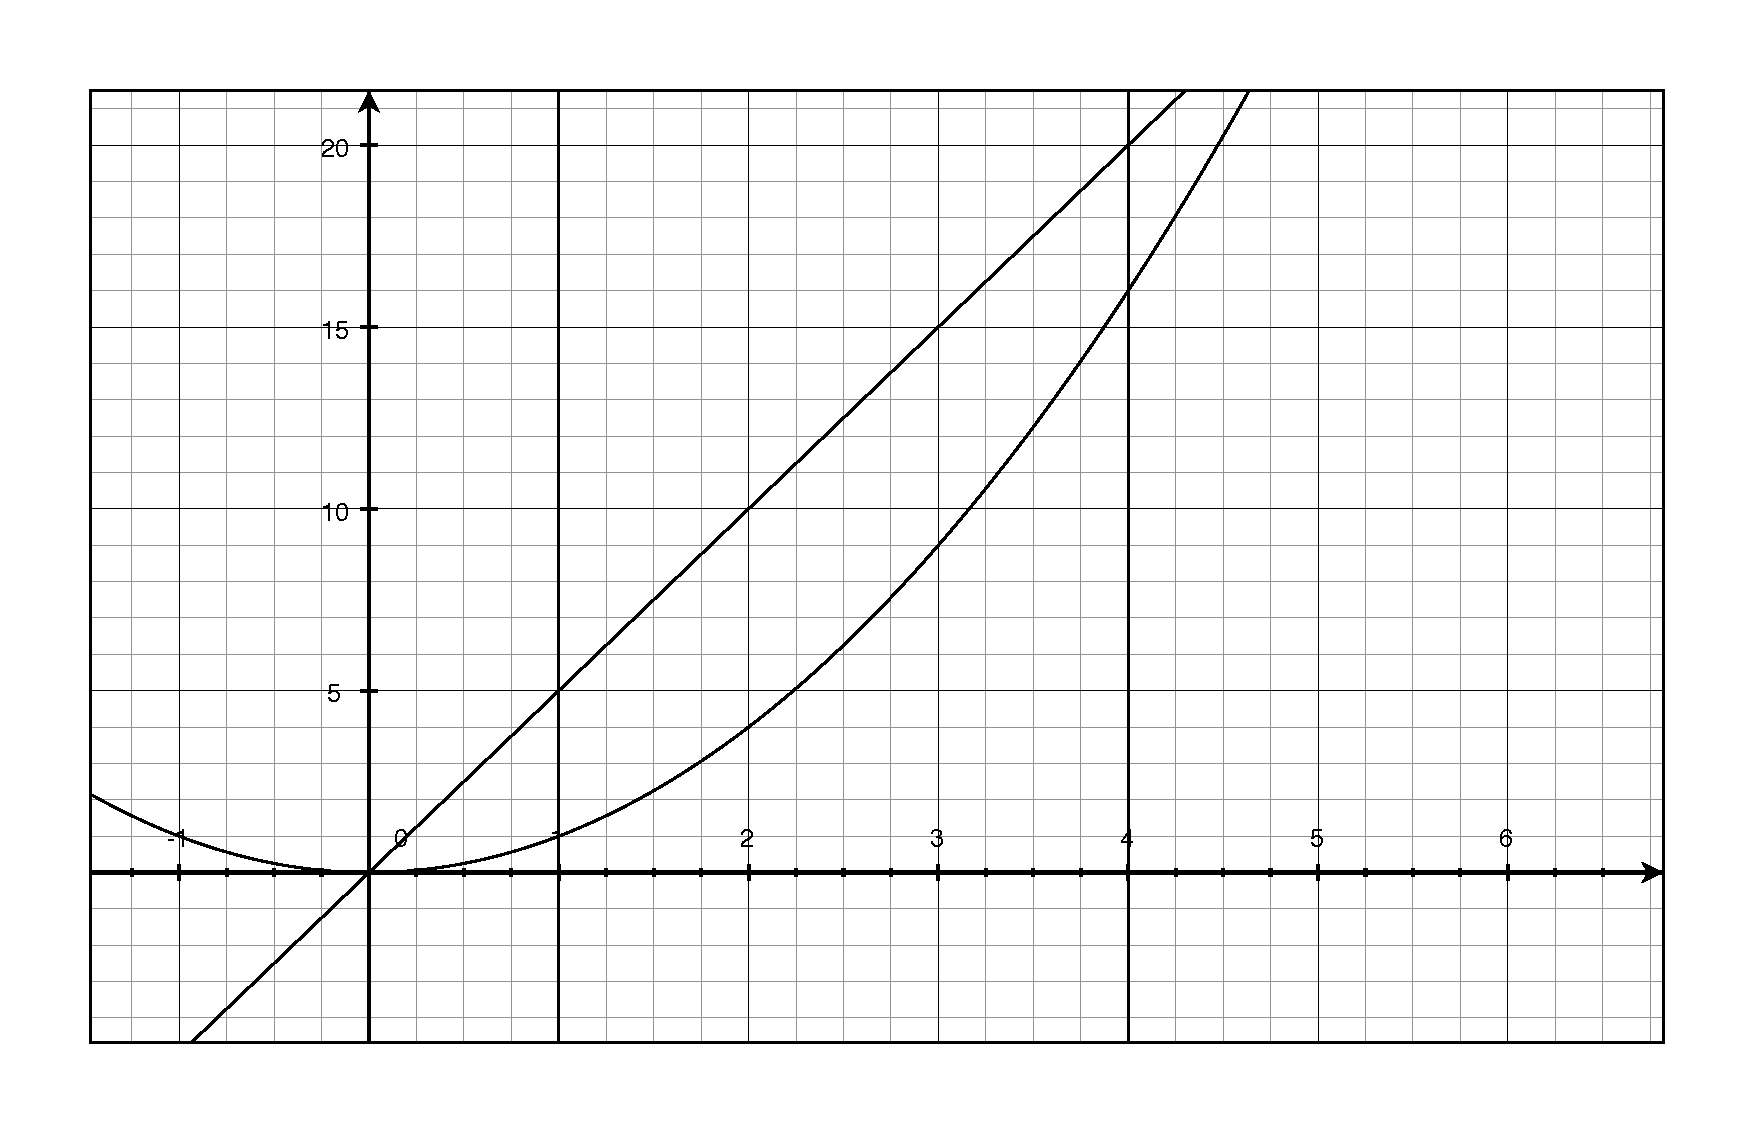
\includegraphics[scale=.3]{extra_credit.eps}
  \caption*{Extra Credit}
\end{figure}

\begin{solution}

The area between $y = 5x$ and the x-axis is:
\[
  A_1 = \int_1^4 5x \, \mathrm{d}x = \frac{5x^2}{2} \bigg|_1^4 = 40 - \frac{5}{2} = \frac{75}{2}
\]

The area between $y = x^2$ and the x-axis is:
\[
  A_1 = \int_1^4 x^2 \, \mathrm{d}x = \frac{x^3}{3} \bigg|_1^4 = \frac{64}{3} - \frac{1}{3} = 21
\]

The desired area is the difference  between these two areas:
\[
  A = \frac{75}{2} - 21 = \frac{33}{2}
\]

\end{solution}

\ifprintanswers
\pagebreak

\section{Section 5.5}

%% \[
%%   \lim_{|P| \to 0} \sum_{n = 1}^n \overline{x}_i^3 \Delta x_i; a = 1, b = 3
%% \]

\begin{description}
\item[7]
\[
  \int_1^3 x^3 \, \mathrm{d}x
\]

\item[8]
\[
  \int_0^2 (x+1)^3 \, \mathrm{d}x
\]

\item[9]
\[
  \int_{-1}^1 \frac{x^2}{1+x} \, \mathrm{d}x
\]

\item[10]
\[
  \int_0^\pi \sin^2 x \, \mathrm{d}x
\]

\item[11]
The interval size is 2, so we need to break the interval into pieces of size $\frac{2}{n}$, starting from $x = 0$.

\begin{align*}
  \int_0^2 (x+1) \, \mathrm{d}x &= \lim_{n \to \infty} \left( \sum_{i = 1}^n \left( \frac{2i}{n} + 1 \right) \cdot \frac{2}{n} \right) \\
  &= \lim_{n \to \infty} \left( \frac{4}{n^2} \sum_{i = 1}^n i + \frac{2}{n} \sum_{i = 1}^n 1 \right) \\
  &= \lim_{n \to \infty} \left( \frac{4}{n^2} \cdot \frac{n(n+1)}{2} + \frac{2}{n} \cdot n \right) \\
  &= \lim_{n \to \infty} \left( 4 + \frac{2}{n^2} \right) \\
  &= 4 \\
\end{align*}

\item[12]
The interval size is 2, so we need to break the interval into pieces of size $\frac{2}{n}$, starting from $x = 0$.

\begin{align*}
  \int_0^2 (x^2+1) \, \mathrm{d}x &= \lim_{n \to \infty} \left( \sum_{i = 1}^n \left[ \left( \frac{2i}{n} \right)^2+ 1 \right] \cdot \frac{2}{n} \right) \\
  &= \lim_{n \to \infty} \left( \frac{8}{n^3} \sum_{i = 1}^n i^2 + \frac{2}{n} \sum_{i = 1}^n 1 \right) \\
  &= \lim_{n \to \infty} \left( \frac{8}{n^3} \cdot \frac{n(n+1)(2n+1)}{6} + \frac{2}{n} \cdot n \right) \\
  &= \lim_{n \to \infty} \left( \frac{8}{3} + \frac{4}{n} + \frac{4}{3n^2} + 2 \right) \\
  &= \frac{14}{3} \\
\end{align*}

\item[13]
The interval size is 3, so we need to break the interval into pieces of size $\frac{3}{n}$, starting from $x = -2$.

\begin{align*}
  \int_{-2}^1 (2x + \pi) \, \mathrm{d}x &= \lim_{n \to \infty} \left( \sum_{i = 1}^n \left[ 2 \left( -2 + \frac{3i}{n} \right) + \pi \right] \cdot \frac{3}{n} \right) \\
  &= 3 \pi - 3 \\
\end{align*}

\item[21]
\begin{enumerate}[a]

\item integrable

\item integrable

\item not integrable---not bounded in interval

\item not integrable---not bounded and not defined for $x = \pm \frac{\pi}{2}$

\item integrable

\item integrable

\end{enumerate}

\end{description}

\pagebreak

\section{5.6}

\begin{description}
\item[1]
\[
   \int_0^2 x^3 \, \mathrm{d}x = \frac{x^4}{4} \, \bigg|_0^2 = 4
\]

\item[2]
\[
   \int_{-1}^2 x^4 \, \mathrm{d}x = \frac{x^5}{5} \, \bigg|_{-1}^2 = \frac{33}{5}
\]

\item[3]
\[
   \int_{-1}^2 \left( 3x^2 - 2x + 3 \right) \, \mathrm{d}x = x^3 - x^2 + 3x \, \bigg|_{-1}^2 = 15
\]

\item[4]
\[
   \int_1^2 \left(4x^3 + 7 \right) \, \mathrm{d}x = x^4 + 7x \, \bigg|_1^2 = 22
\]

\item[5]
\[
   \int_1^2 w^{-2} \, \mathrm{d}w = -w^{-1} \, \bigg|_1^2 = \frac{3}{4}
\]

\item[6]
\[
   \int_1^3 2t^{-3} \, \mathrm{d}t = -t^{-2} \, \bigg|_1^3 = \frac{8}{9}
\]

\item[7]
\[
   \int_0^4 t^{1/2} \, \mathrm{d}t = \frac{2}{3} t^{3/2} \, \bigg|_0^4 = \frac{16}{3}
\]

\item[8]
\[
   \int_1^8 w^{1/3} \, \mathrm{d}w = \frac{3}{4} w^{4/3} \, \bigg|_1^8 = \frac{45}{4}
\]

\item[9]
\begin{align*}
  \int_{-4}^{-2} \left(y^2 + y^{-3} \right) \, \mathrm{d}y &= \frac{y^3}{3} - \frac{1}{2y^2} \, \bigg|_{-4}^{-2} \\
  &= \frac{-8}{3} - \frac{1}{8} - \left( \frac{-64}{3} - \frac{1}{32} \right) \\
  %% &= \frac{-67}{24} - \left( \frac{-2,051}{96} \right) \\
  %% &= \frac{-67}{24} - \left( \frac{-2,051}{96} \right) \\
  %% &= \frac{-268}{96} - \left( \frac{-2,051}{96} \right) \\
  &= -\frac{1,783}{96} \\
\end{align*}

\item[10]
\begin{align*}
  \int_1^4 \frac{s^4 - 8}{s^2} \, \mathrm{d}s &= \int_1^4 \left( s^2 - 8s^{-2} \right) \, \mathrm{d}s \\
  &= \frac{s^3}{3} + \frac{8}{s} \, \bigg|_1^4 \\
  &= \frac{64}{3} + \frac{8}{4} - \left( \frac{1}{3} + 8 \right) \\
  &= 15 \\
\end{align*}

\item[11]
\[
   \int_0^{\pi/2} \cos x \, \mathrm{d}x = \sin x \, \bigg|_0^{\pi/2} = 1
\]

\item[12]
\[
   \int_{\pi/6}^{\pi/2} 2 \sin t \, \mathrm{d}t = -2 \cos x \, \bigg|_{\pi/6}^{\pi/2} = \sqrt{3}
\]

\item[13]
\[
   \int_0^1 \left( 2x^4 - 3x^2 + 5 \right) \, \mathrm{d}x = \frac{2x^5}{5} - x^3 + 5x \, \bigg|_0^1 = \frac{22}{5}
\]

\item[14]
\[
   \int_0^1 \left( x^{4/3} - 2x^{1/3} \right) \, \mathrm{d}x = \frac{3x^{7/3}}{7} - \frac{3x^{4/3}}{2}\, \bigg|_0^1 = - \frac{15}{4}
\]

\item[31]
\[
   \int_0^3 x^2 \, \mathrm{d}x = \frac{1}{3} x^3 \bigg|_0^3 = 9
\]

\item[32]
\[
   \int_0^2 x^3 \, \mathrm{d}x = \frac{1}{4} x^4 \bigg|_0^2 = 4
\]



\end{description}

\else

% \vspace{2 cm}

{Crooked is the path of eternity}
\vspace{.2 cm}

\hspace{0.5 cm} --Friedrich Nietzsche

%% {\em Some writers have so confounded society with government, as to leave little or no distinction between them; whereas
%%   they are not only different, but have different origins. Society is produced by our wants, and government by our
%%   wickedness; the former promotes our happiness POSITIVELY by uniting our affections, the latter NEGATIVELY by
%%   restraining our vices. The one encourages intercourse, the other creates distinctions. The first a patron, the last a
%%   punisher.} --Thomas Paine

%% {\em I build no system. I ask an end to privilege, the abolition of slavery, equality of rights, and the reign of
%% law. Justice, nothing else; that is the alpha and omega of my argument: to others I leave the business of governing the
%% world.}

%% \vspace{.2 cm}

%% \hspace{1 cm} --Pierre-Joseph Proudhon

\fi

\end{document}

